\documentclass[]{article}
\usepackage{lmodern}
\usepackage{amssymb,amsmath}
\usepackage{ifxetex,ifluatex}
\usepackage{fixltx2e} % provides \textsubscript
\ifnum 0\ifxetex 1\fi\ifluatex 1\fi=0 % if pdftex
  \usepackage[T1]{fontenc}
  \usepackage[utf8]{inputenc}
\else % if luatex or xelatex
  \ifxetex
    \usepackage{mathspec}
  \else
    \usepackage{fontspec}
  \fi
  \defaultfontfeatures{Ligatures=TeX,Scale=MatchLowercase}
\fi
% use upquote if available, for straight quotes in verbatim environments
\IfFileExists{upquote.sty}{\usepackage{upquote}}{}
% use microtype if available
\IfFileExists{microtype.sty}{%
\usepackage{microtype}
\UseMicrotypeSet[protrusion]{basicmath} % disable protrusion for tt fonts
}{}
\usepackage[margin=1in]{geometry}
\usepackage{hyperref}
\hypersetup{unicode=true,
            pdftitle={FlipTheFleet Black Box Data Tests},
            pdfauthor={Ben Anderson (b.anderson@soton.ac.uk, @dataknut)},
            pdfborder={0 0 0},
            breaklinks=true}
\urlstyle{same}  % don't use monospace font for urls
\usepackage{color}
\usepackage{fancyvrb}
\newcommand{\VerbBar}{|}
\newcommand{\VERB}{\Verb[commandchars=\\\{\}]}
\DefineVerbatimEnvironment{Highlighting}{Verbatim}{commandchars=\\\{\}}
% Add ',fontsize=\small' for more characters per line
\usepackage{framed}
\definecolor{shadecolor}{RGB}{248,248,248}
\newenvironment{Shaded}{\begin{snugshade}}{\end{snugshade}}
\newcommand{\KeywordTok}[1]{\textcolor[rgb]{0.13,0.29,0.53}{\textbf{#1}}}
\newcommand{\DataTypeTok}[1]{\textcolor[rgb]{0.13,0.29,0.53}{#1}}
\newcommand{\DecValTok}[1]{\textcolor[rgb]{0.00,0.00,0.81}{#1}}
\newcommand{\BaseNTok}[1]{\textcolor[rgb]{0.00,0.00,0.81}{#1}}
\newcommand{\FloatTok}[1]{\textcolor[rgb]{0.00,0.00,0.81}{#1}}
\newcommand{\ConstantTok}[1]{\textcolor[rgb]{0.00,0.00,0.00}{#1}}
\newcommand{\CharTok}[1]{\textcolor[rgb]{0.31,0.60,0.02}{#1}}
\newcommand{\SpecialCharTok}[1]{\textcolor[rgb]{0.00,0.00,0.00}{#1}}
\newcommand{\StringTok}[1]{\textcolor[rgb]{0.31,0.60,0.02}{#1}}
\newcommand{\VerbatimStringTok}[1]{\textcolor[rgb]{0.31,0.60,0.02}{#1}}
\newcommand{\SpecialStringTok}[1]{\textcolor[rgb]{0.31,0.60,0.02}{#1}}
\newcommand{\ImportTok}[1]{#1}
\newcommand{\CommentTok}[1]{\textcolor[rgb]{0.56,0.35,0.01}{\textit{#1}}}
\newcommand{\DocumentationTok}[1]{\textcolor[rgb]{0.56,0.35,0.01}{\textbf{\textit{#1}}}}
\newcommand{\AnnotationTok}[1]{\textcolor[rgb]{0.56,0.35,0.01}{\textbf{\textit{#1}}}}
\newcommand{\CommentVarTok}[1]{\textcolor[rgb]{0.56,0.35,0.01}{\textbf{\textit{#1}}}}
\newcommand{\OtherTok}[1]{\textcolor[rgb]{0.56,0.35,0.01}{#1}}
\newcommand{\FunctionTok}[1]{\textcolor[rgb]{0.00,0.00,0.00}{#1}}
\newcommand{\VariableTok}[1]{\textcolor[rgb]{0.00,0.00,0.00}{#1}}
\newcommand{\ControlFlowTok}[1]{\textcolor[rgb]{0.13,0.29,0.53}{\textbf{#1}}}
\newcommand{\OperatorTok}[1]{\textcolor[rgb]{0.81,0.36,0.00}{\textbf{#1}}}
\newcommand{\BuiltInTok}[1]{#1}
\newcommand{\ExtensionTok}[1]{#1}
\newcommand{\PreprocessorTok}[1]{\textcolor[rgb]{0.56,0.35,0.01}{\textit{#1}}}
\newcommand{\AttributeTok}[1]{\textcolor[rgb]{0.77,0.63,0.00}{#1}}
\newcommand{\RegionMarkerTok}[1]{#1}
\newcommand{\InformationTok}[1]{\textcolor[rgb]{0.56,0.35,0.01}{\textbf{\textit{#1}}}}
\newcommand{\WarningTok}[1]{\textcolor[rgb]{0.56,0.35,0.01}{\textbf{\textit{#1}}}}
\newcommand{\AlertTok}[1]{\textcolor[rgb]{0.94,0.16,0.16}{#1}}
\newcommand{\ErrorTok}[1]{\textcolor[rgb]{0.64,0.00,0.00}{\textbf{#1}}}
\newcommand{\NormalTok}[1]{#1}
\usepackage{longtable,booktabs}
\usepackage{graphicx,grffile}
\makeatletter
\def\maxwidth{\ifdim\Gin@nat@width>\linewidth\linewidth\else\Gin@nat@width\fi}
\def\maxheight{\ifdim\Gin@nat@height>\textheight\textheight\else\Gin@nat@height\fi}
\makeatother
% Scale images if necessary, so that they will not overflow the page
% margins by default, and it is still possible to overwrite the defaults
% using explicit options in \includegraphics[width, height, ...]{}
\setkeys{Gin}{width=\maxwidth,height=\maxheight,keepaspectratio}
\IfFileExists{parskip.sty}{%
\usepackage{parskip}
}{% else
\setlength{\parindent}{0pt}
\setlength{\parskip}{6pt plus 2pt minus 1pt}
}
\setlength{\emergencystretch}{3em}  % prevent overfull lines
\providecommand{\tightlist}{%
  \setlength{\itemsep}{0pt}\setlength{\parskip}{0pt}}
\setcounter{secnumdepth}{5}
% Redefines (sub)paragraphs to behave more like sections
\ifx\paragraph\undefined\else
\let\oldparagraph\paragraph
\renewcommand{\paragraph}[1]{\oldparagraph{#1}\mbox{}}
\fi
\ifx\subparagraph\undefined\else
\let\oldsubparagraph\subparagraph
\renewcommand{\subparagraph}[1]{\oldsubparagraph{#1}\mbox{}}
\fi

%%% Use protect on footnotes to avoid problems with footnotes in titles
\let\rmarkdownfootnote\footnote%
\def\footnote{\protect\rmarkdownfootnote}

%%% Change title format to be more compact
\usepackage{titling}

% Create subtitle command for use in maketitle
\newcommand{\subtitle}[1]{
  \posttitle{
    \begin{center}\large#1\end{center}
    }
}

\setlength{\droptitle}{-2em}

  \title{FlipTheFleet Black Box Data Tests}
    \pretitle{\vspace{\droptitle}\centering\huge}
  \posttitle{\par}
  \subtitle{Testing Time of Charging}
  \author{Ben Anderson
(\href{mailto:b.anderson@soton.ac.uk}{\nolinkurl{b.anderson@soton.ac.uk}},
\texttt{@dataknut})}
    \preauthor{\centering\large\emph}
  \postauthor{\par}
      \predate{\centering\large\emph}
  \postdate{\par}
    \date{Last run at: 2018-10-26 15:36:22}

\usepackage{booktabs}
\usepackage{longtable}
\usepackage{array}
\usepackage{multirow}
\usepackage[table]{xcolor}
\usepackage{wrapfig}
\usepackage{float}
\usepackage{colortbl}
\usepackage{pdflscape}
\usepackage{tabu}
\usepackage{threeparttable}
\usepackage{threeparttablex}
\usepackage[normalem]{ulem}
\usepackage{makecell}

\begin{document}
\maketitle

{
\setcounter{tocdepth}{2}
\tableofcontents
}
\newpage

\section{Citation}\label{citation}

If you wish to use any of the material from this report please cite as:

\begin{itemize}
\tightlist
\item
  Anderson, B. (2018) \emph{FlipTheFleet Black Box Data Tests: Testing
  Time of Charging},
  \href{http://www.otago.ac.nz/centre-sustainability/}{Centre for
  Sustainability}, University of Otago: Dunedin, New Zealand.
\end{itemize}

This work is (c) 2018 the University of Southampton. Re-use is governed
by \href{https://github.com/CfSOtago/GREENGrid/blob/master/LICENSE}{this
license}.

\newpage

\section{About}\label{about}

\subsection{Circulation}\label{circulation}

Report circulation:

\begin{itemize}
\tightlist
\item
  Restricted to:
  \href{https://www.otago.ac.nz/centre-sustainability/research/energy/otago050285.html}{NZ
  GREEN Grid} project partners and contractors.
\end{itemize}

\subsection{Purpose}\label{purpose}

This report is intended to:

\begin{itemize}
\tightlist
\item
  load and test preliminary
  `\href{https://flipthefleet.org/ev-black-box/}{black box}' (see Figure
  \ref{fig:blackBox}) EV monitoring data provided for assessment
  purposes by \href{http://flipthefleet.org/}{FlipTheFleet}
\item
  preliminary analysis of time of charging to understand impact on
  `peak' electricity demand
\end{itemize}

\begin{figure}

\hfill{}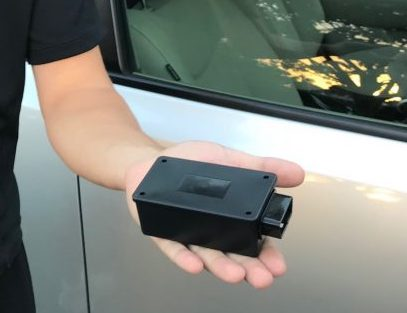
\includegraphics[width=4.24in]{fig/bb} 

\caption{The Black Box (Source: FlipTheFleet)}\label{fig:blackBox}
\end{figure}

\subsection{Requirements:}\label{requirements}

\begin{itemize}
\tightlist
\item
  test FlipTheFleet black box dataset stored on the University of
  Otago's High-Capacity Central File Storage
  \href{https://www.otago.ac.nz/its/services/hosting/otago068353.html}{HCS}
  at: /Volumes/hum-csafe/Research Projects/GREEN
  Grid/externalData/flipTheFleet/safe/ftfSafeLatestAll.csv.gz
\end{itemize}

\subsection{Code and report history}\label{code-and-report-history}

Generally tracked via our git.soton
\href{https://git.soton.ac.uk/ba1e12/nzGREENGrid}{repo}:

\begin{itemize}
\tightlist
\item
  \href{https://git.soton.ac.uk/ba1e12/nzGREENGrid/commits/master}{history}
\item
  \href{https://git.soton.ac.uk/ba1e12/nzGREENGrid/issues}{issues}
\end{itemize}

Specific history of this code:

\begin{itemize}
\tightlist
\item
  \url{https://git.soton.ac.uk/ba1e12/nzGREENGrid/tree/master/analysis/ev}
\end{itemize}

\subsection{Support}\label{support}

This work was supported by:

\begin{itemize}
\tightlist
\item
  The \href{https://www.otago.ac.nz/}{University of Otago};
\item
  The \href{https://www.southampton.ac.uk/}{University of Southampton};
\item
  The New Zealand \href{http://www.mbie.govt.nz/}{Ministry of Business,
  Innovation and Employment (MBIE)} through the
  \href{https://www.otago.ac.nz/centre-sustainability/research/energy/otago050285.html}{NZ
  GREEN Grid} project;
\item
  \href{http://www.energy.soton.ac.uk/tag/spatialec/}{SPATIALEC} - a
  \href{http://ec.europa.eu/research/mariecurieactions/about-msca/actions/if/index_en.htm}{Marie
  Skłodowska-Curie Global Fellowship} based at the University of Otago's
  \href{http://www.otago.ac.nz/centre-sustainability/staff/otago673896.html}{Centre
  for Sustainability} (2017-2019) \& the University of Southampton's
  Sustainable Energy Research Group (2019-2020).
\end{itemize}

We do not `support' the code but if you notice a problem please check
the \href{https://github.com/CfSOtago/GREENGrid/issues}{issues} on our
\href{https://github.com/CfSOtago/GREENGrid}{repo} and if it doesn't
already exist, please open a new one.

\subsection{Notes}\label{notes}

This document was created using
\href{https://cran.r-project.org/package=knitr}{knitr} in
\href{http://www.rstudio.com}{RStudio} with R version 3.5.1 (2018-07-02)
running on x86\_64-apple-darwin15.6.0. Some of the R code has been
included where used for information and reference purposes. Full code is
\href{https://github.com/CfSOtago/GREENGrid/tree/master/analysis/ev}{available}
as noted above.

\section{Load and check data}\label{load-and-check-data}

\subsection{Load data}\label{load-data}

In this section we load and describe the pre-processed safe data from
/Volumes/hum-csafe/Research Projects/GREEN
Grid/externalData/flipTheFleet/safe/ftfSafeLatestAll.csv.gz. Note that
this data does \emph{not} contain Latitude/Longitude or the vehicle
registration number. This has been replaced by a unique hash code (per
vehicle).

\begin{Shaded}
\begin{Highlighting}[]
\NormalTok{ftfSafeDT <-}\StringTok{ }\NormalTok{data.table}\OperatorTok{::}\KeywordTok{as.data.table}\NormalTok{(readr}\OperatorTok{::}\KeywordTok{read_csv}\NormalTok{(dFile))}
\end{Highlighting}
\end{Shaded}

\begin{verbatim}
## Parsed with column specification:
## cols(
##   .default = col_integer(),
##   `Date (GPS)` = col_character(),
##   Altitude = col_double(),
##   `Speed (GPS)` = col_double(),
##   `Speed (Speedometer)` = col_double(),
##   SOC = col_double(),
##   AHr = col_double(),
##   `Pack volts` = col_double(),
##   `Pack amps` = col_double(),
##   `Pack 1 temp (C)` = col_double(),
##   `Pack 2 temp (C)` = col_double(),
##   `Pack 3 temp (C)` = col_double(),
##   `Pack 4 temp (C)` = col_double(),
##   `12V battery (amps)` = col_double(),
##   Hx = col_double(),
##   VIN = col_character(),
##   `12V battery (volts)` = col_double(),
##   `ACC (V)` = col_double(),
##   SOH = col_double(),
##   `SOH (version 2)` = col_double(),
##   `Charger (amps)` = col_double()
##   # ... with 88 more columns
## )
\end{verbatim}

\begin{verbatim}
## See spec(...) for full column specifications.
\end{verbatim}

\begin{verbatim}
## Warning in rbind(names(probs), probs_f): number of columns of result is not
## a multiple of vector length (arg 1)
\end{verbatim}

\begin{verbatim}
## Warning: 11793 parsing failures.
## row # A tibble: 5 x 5 col     row col      expected       actual    file                             expected   <int> <chr>    <chr>          <chr>     <chr>                            actual 1 12490 cabin_t~ no trailing c~ .6666666~ '/Volumes/hum-csafe/Research Pr~ file 2 12494 cabin_t~ no trailing c~ .6666666~ '/Volumes/hum-csafe/Research Pr~ row 3 12496 cabin_t~ no trailing c~ .6666666~ '/Volumes/hum-csafe/Research Pr~ col 4 12499 cabin_t~ no trailing c~ .2222222~ '/Volumes/hum-csafe/Research Pr~ expected 5 12501 cabin_t~ no trailing c~ .2222222~ '/Volumes/hum-csafe/Research Pr~
## ... ................. ... .......................................................................... ........ .......................................................................... ...... .......................................................................... .... .......................................................................... ... .......................................................................... ... .......................................................................... ........ ..........................................................................
## See problems(...) for more details.
\end{verbatim}

\begin{Shaded}
\begin{Highlighting}[]
\CommentTok{# re-create rTime}
\NormalTok{ftfSafeDT <-}\StringTok{ }\NormalTok{ftfSafeDT[, rTime }\OperatorTok{:}\ErrorTok{=}\StringTok{ }\NormalTok{hms}\OperatorTok{::}\KeywordTok{as.hms}\NormalTok{(rDateTime)]}

\CommentTok{# re-create rDow to stop it acting like a factor with alphabetic ordering}
\NormalTok{ftfSafeDT <-}\StringTok{ }\NormalTok{ftfSafeDT[, rDow }\OperatorTok{:}\ErrorTok{=}\StringTok{ }\NormalTok{lubridate}\OperatorTok{::}\KeywordTok{wday}\NormalTok{(rDateTime, }\DataTypeTok{lab =} \OtherTok{TRUE}\NormalTok{)]}
\end{Highlighting}
\end{Shaded}

That loaded 46,741 observations from 2 vehicles. Table
\ref{tab:evSummary} summarises the available data for each EV.

\begin{table}

\caption{\label{tab:evSummary}Start and end of observation period and number of obs by anonymised vehicle ID}
\centering
\begin{tabular}[t]{l|l|l|r}
\hline
evID & obsStart & obsEnd & nObservations\\
\hline
44e70b238906b67964c088be78366d2c & 2018-07-12 11:02:49 & 2018-09-08 15:27:48 & 34254\\
\hline
b4ed70fa9b8d2419411908df6d78ee2a & 2018-05-01 12:42:27 & 2018-06-11 09:40:28 & 12487\\
\hline
\end{tabular}
\end{table}

\subsection{Check data quality}\label{check-data-quality}

Next we check for NA in dates and other key variables.

\begin{table}

\caption{\label{tab:checkVolts}Number of obs and mean pack volts where date cannot be set by original GPS Date and Time}
\centering
\begin{tabular}[t]{l|r|r|r}
\hline
Date (GPS) & Time (GPS) & nObs & meanPackVolts\\
\hline
NA & NA & 17472 & 90.15239\\
\hline
\end{tabular}
\end{table}

\begin{table}

\caption{\label{tab:checkAmps}Number of obs and mean pack amps where time cannot be set by original GPS Date and Time}
\centering
\begin{tabular}[t]{l|r|r|r}
\hline
Date (GPS) & Time (GPS) & nObs & meanPackAmps\\
\hline
NA & NA & 17472 & 16.5822\\
\hline
\end{tabular}
\end{table}

It looks like there are NAs in the GPS derived Date \& Time variables.

Since we really need to know the date and time, we remove these NAs from
the data although they comprise 17472 (37.38 \%) observations.

\begin{quote}
\emph{XX (should we remove them - what does GPS NA mean? no signal?) XX
}
\end{quote}

\subsection{Check variables of interest for this
analysis}\label{check-variables-of-interest-for-this-analysis}

Check charger related variables. These are:

\begin{itemize}
\tightlist
\item
  \texttt{Pack\ amps}
\item
  \texttt{Pack\ volts}
\end{itemize}

\begin{quote}
DM: ``To determine charger power the variables `Pack volts' and `Pack
amps' give you everything you need (with some extra code to separate out
regen, and it is also useful to do some deltas of voltage and SoC over
time to deal with noise in the current sensors). Negative pack amps with
speed also at zero is charging (speed greater than zero and negative
pack amps is regen).''
\end{quote}

Multiplying these two will give power in W. Figures
\ref{fig:checkAmpDist} to \ref{fig:checkPowerDist} examine the
distribution of amps, volts and the derived W.

Figure \ref{fig:checkAmpDist} shows a density plot for pack amps by EV
and by whether or not the amps are -ve, +ve or 0. As we can see,
positive amps (providing power to the vehicle) has a cluster of readings
close to 0 and then a long positive tail. Negative amps (re-charging the
battery) appears to have two distinct clusters and a similarly long
negative tail. Only one vehicle reports a large number of 0 Amp
readings.

\begin{table}

\caption{\label{tab:checkAmpDist}Amps check}
\centering
\begin{tabular}[t]{l|l|r|r|r|r}
\hline
ampFlag & evID & nObs & max & mean & min\\
\hline
Negative amps & 44e70b238906b67964c088be78366d2c & 14415 & -0.001 & -8.029587 & -125.991\\
\hline
Negative amps & b4ed70fa9b8d2419411908df6d78ee2a & 9522 & -0.001 & -8.377448 & -32.754\\
\hline
Positive amps & 44e70b238906b67964c088be78366d2c & 3524 & 214.546 & 30.152265 & 0.001\\
\hline
Positive amps & b4ed70fa9b8d2419411908df6d78ee2a & 1624 & 32.747 & 10.534372 & 0.002\\
\hline
Zero amps & 44e70b238906b67964c088be78366d2c & 3 & 0.000 & 0.000000 & 0.000\\
\hline
Zero amps & b4ed70fa9b8d2419411908df6d78ee2a & 181 & 0.000 & 0.000000 & 0.000\\
\hline
\end{tabular}
\end{table}

\begin{figure}
\centering
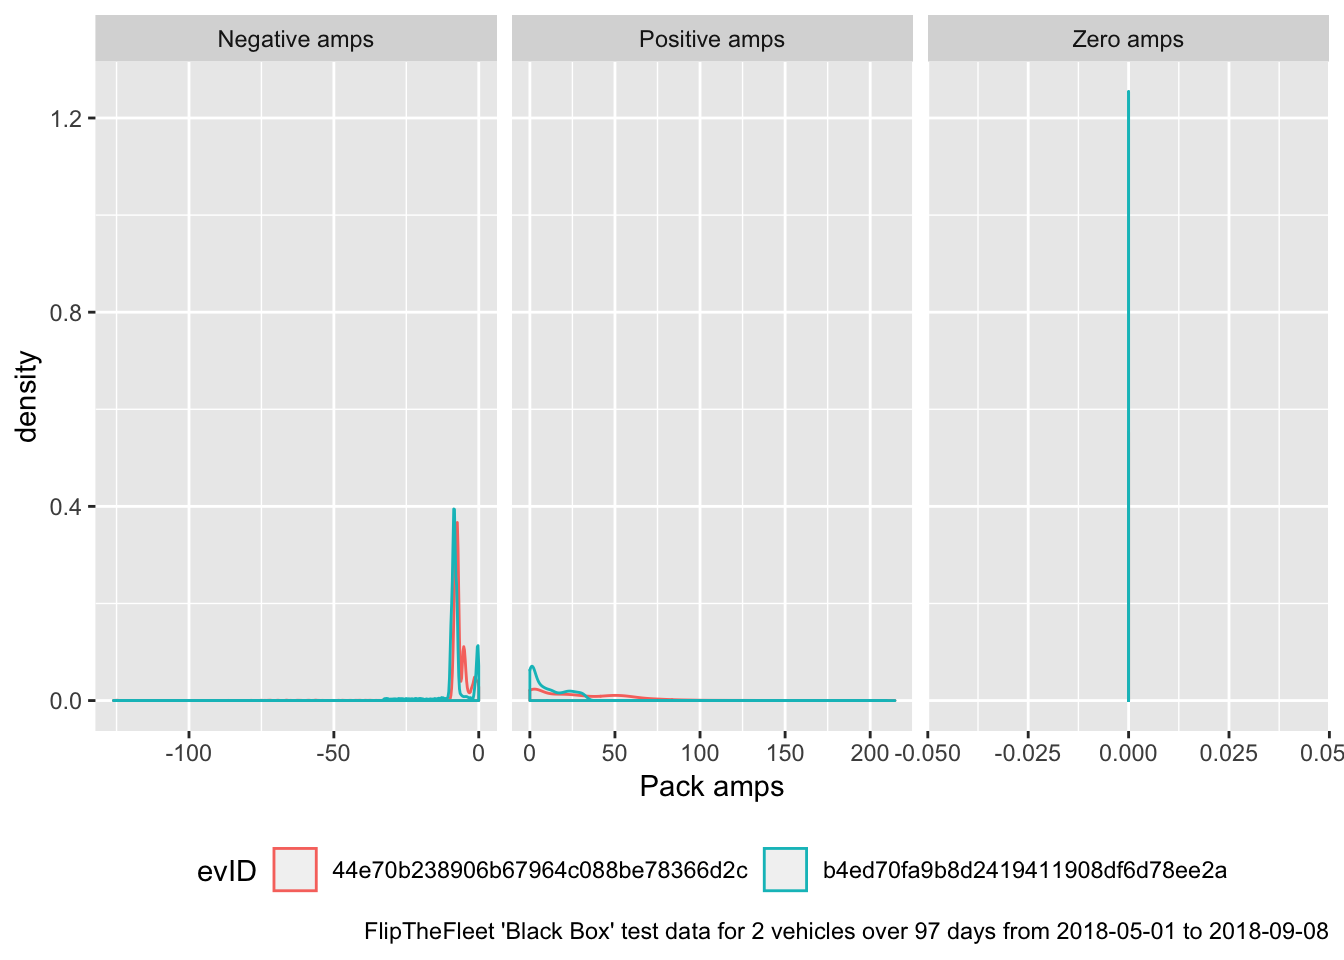
\includegraphics{ftFBlackBoxTestDataChargeTime_files/figure-latex/checkAmpDist-1.pdf}
\caption{\label{fig:checkAmpDist}Distribution of Pack amp readings by car}
\end{figure}

Next we check volts. Again we seperate -ve and +ve values. In this case
it appears that we should probably filter out:

\begin{itemize}
\tightlist
\item
  -ve volts
\item
  volts \textgreater{} 1000
\end{itemize}

\begin{table}

\caption{\label{tab:checkVoltsDist}Volts check}
\centering
\begin{tabular}[t]{l|l|r|r|r|r}
\hline
voltFlag & evID & nObs & max & mean & min\\
\hline
Negative volts & 44e70b238906b67964c088be78366d2c & 8 & 0.000 & 0.0000 & 0.000\\
\hline
Negative volts & b4ed70fa9b8d2419411908df6d78ee2a & 87 & 0.000 & 0.0000 & 0.000\\
\hline
Positive volts & 44e70b238906b67964c088be78366d2c & 17934 & 397.056 & 382.9832 & 340.320\\
\hline
Positive volts & b4ed70fa9b8d2419411908df6d78ee2a & 11240 & 5783.520 & 430.0139 & 269.856\\
\hline
\end{tabular}
\end{table}

\begin{figure}
\centering
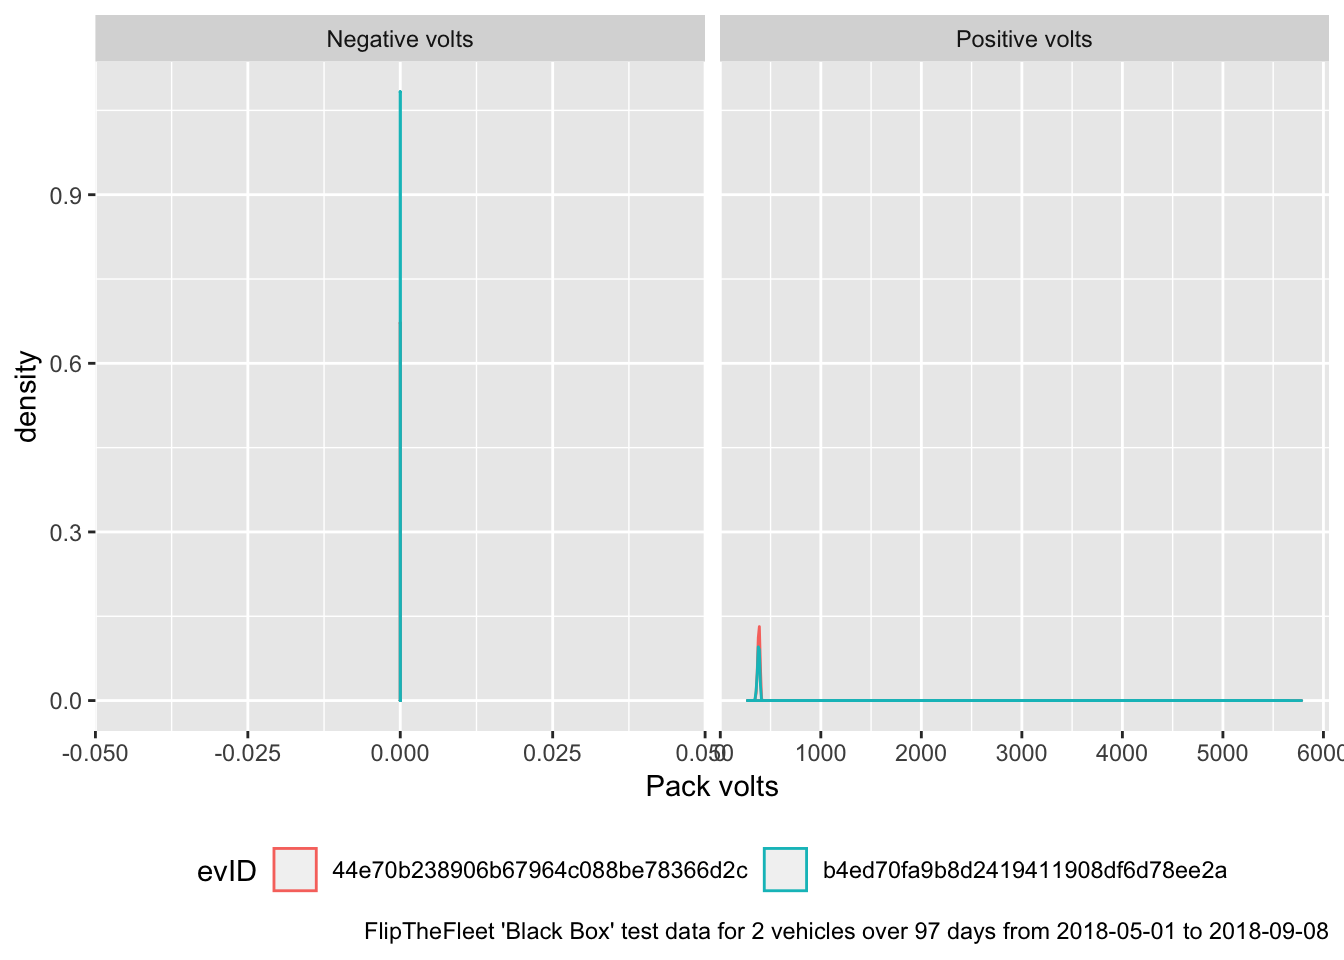
\includegraphics{ftFBlackBoxTestDataChargeTime_files/figure-latex/checkVoltsDist-1.pdf}
\caption{\label{fig:checkVoltsDist}Distribution of charger volt readings}
\end{figure}

Finally (Figure \ref{fig:checkPowerDist}) shows the distirbution of the
derived -ve, zero and +ve power values using the following filters:

\begin{itemize}
\tightlist
\item
  volts \textless{} 0 and volts \textgreater{} 1000 = ``Volt error?''
\end{itemize}

\begin{table}

\caption{\label{tab:checkPowerDist}Power check}
\centering
\begin{tabular}[t]{l|l|r|r|r|r}
\hline
powerFlag & evID & nObs & max & mean & min\\
\hline
Negative power & 44e70b238906b67964c088be78366d2c & 14411 & -0.396384 & -3077.387 & -49196.687616\\
\hline
Negative power & b4ed70fa9b8d2419411908df6d78ee2a & 9318 & -0.383712 & -3197.947 & -12530.626560\\
\hline
Positive power & 44e70b238906b67964c088be78366d2c & 3520 & 82266.190464 & 11284.541 & 0.396576\\
\hline
Positive power & b4ed70fa9b8d2419411908df6d78ee2a & 1611 & 12831.848640 & 3936.218 & 0.740352\\
\hline
Volt error? & 44e70b238906b67964c088be78366d2c & 8 & NA & NA & NA\\
\hline
Volt error? & b4ed70fa9b8d2419411908df6d78ee2a & 280 & NA & NA & NA\\
\hline
Zero power & 44e70b238906b67964c088be78366d2c & 3 & 0.000000 & 0.000 & 0.000000\\
\hline
Zero power & b4ed70fa9b8d2419411908df6d78ee2a & 118 & 0.000000 & 0.000 & 0.000000\\
\hline
\end{tabular}
\end{table}

\begin{verbatim}
## `stat_bin()` using `bins = 30`. Pick better value with `binwidth`.
\end{verbatim}

\begin{verbatim}
## Warning: Removed 288 rows containing non-finite values (stat_bin).
\end{verbatim}

\begin{figure}
\centering
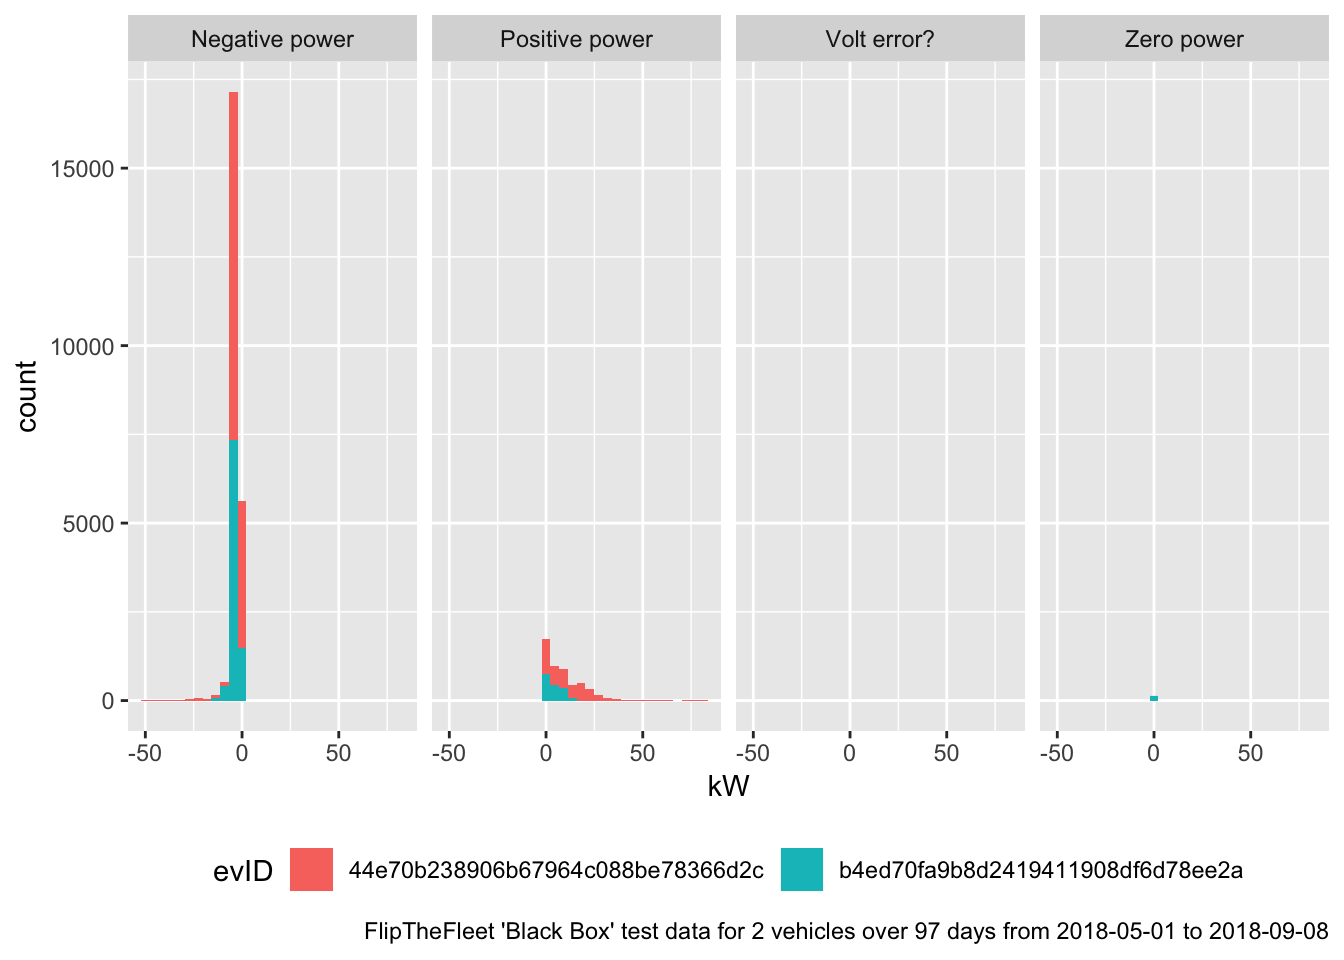
\includegraphics{ftFBlackBoxTestDataChargeTime_files/figure-latex/checkPowerDist-1.pdf}
\caption{\label{fig:checkPowerDist}Distribution of derived power demand
using these filters}
\end{figure}

As noted above, battery charging will be occuring when power is
negative. This will be from the grid when speed is zero.

\section{Analysis: Number of observations over
time}\label{analysis-number-of-observations-over-time}

Just a simple trend line for each vehicle\ldots{} Note that the
\texttt{Reg\ No} has been replaced with a unique hash ID.

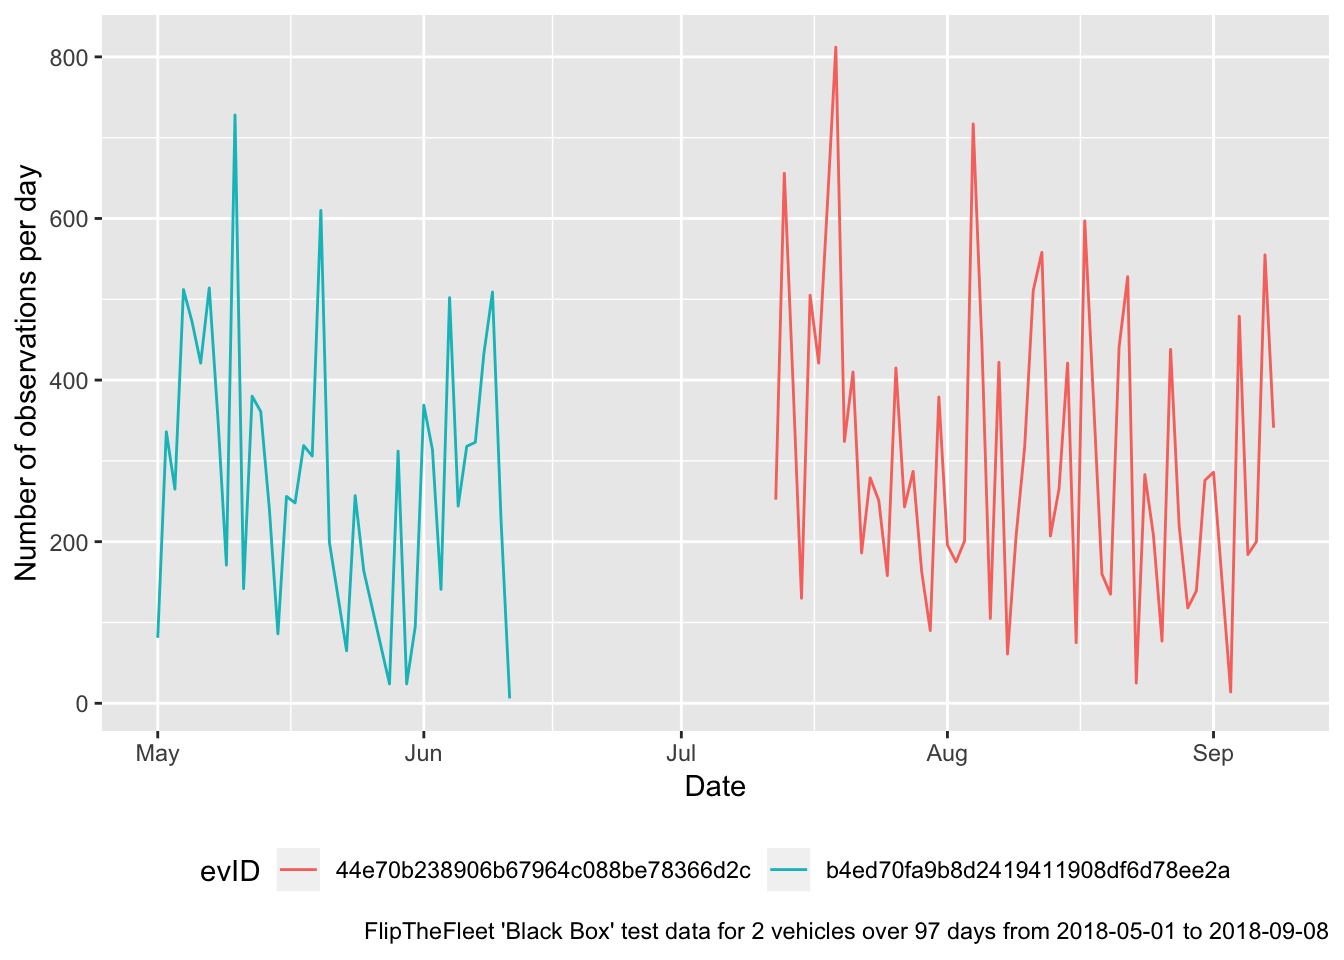
\includegraphics{ftFBlackBoxTestDataChargeTime_files/figure-latex/carTrends-1.pdf}

\section{Analysis: Power flows to/from
batteries}\label{analysis-power-flows-tofrom-batteries}

We use \texttt{Speed\ (Speedometer)} as this has no missing values
(unlike \texttt{Speed\ (GPS)}) to flag observations which should be
electricity grid based as opposed to regenerative charging.

\begin{table}

\caption{\label{tab:powerTable}Check coding}
\centering
\begin{tabular}[t]{l|r|r|r}
\hline
chargingFlag & minSpeed & meanSpeed & maxSpeed\\
\hline
Vehicle in use (no charging)? & 0.00 & 41.60903 & 111.82\\
\hline
Regenerative? & 2.87 & 51.16671 & 101.97\\
\hline
Grid? & 0.00 & 0.00000 & 0.00\\
\hline
\end{tabular}
\end{table}

\begin{table}

\caption{\label{tab:powerTable}Summary of derived chargeingPowerW per car}
\centering
\begin{tabular}[t]{l|l|r|r|r}
\hline
evID & chargingFlag & meankW & sdkW & mediankW\\
\hline
44e70b238906b67964c088be78366d2c & Grid? & -2.786912 & 3.229894 & -2.816239\\
\hline
44e70b238906b67964c088be78366d2c & Regenerative? & -9.053428 & 8.645677 & -6.050238\\
\hline
44e70b238906b67964c088be78366d2c & Vehicle in use (no charging)? & NA & NA & NA\\
\hline
b4ed70fa9b8d2419411908df6d78ee2a & Grid? & -2.833136 & 1.224567 & -3.179782\\
\hline
b4ed70fa9b8d2419411908df6d78ee2a & Regenerative? & -5.895578 & 3.447599 & -5.543476\\
\hline
b4ed70fa9b8d2419411908df6d78ee2a & Vehicle in use (no charging)? & NA & NA & NA\\
\hline
\end{tabular}
\end{table}

Figure \ref{fig:chargingHisto} shows the expected clustering of
grid-based charging in the \textless{} 5 kW region.

\begin{verbatim}
## Warning: Removed 288 rows containing non-finite values (stat_density).
\end{verbatim}

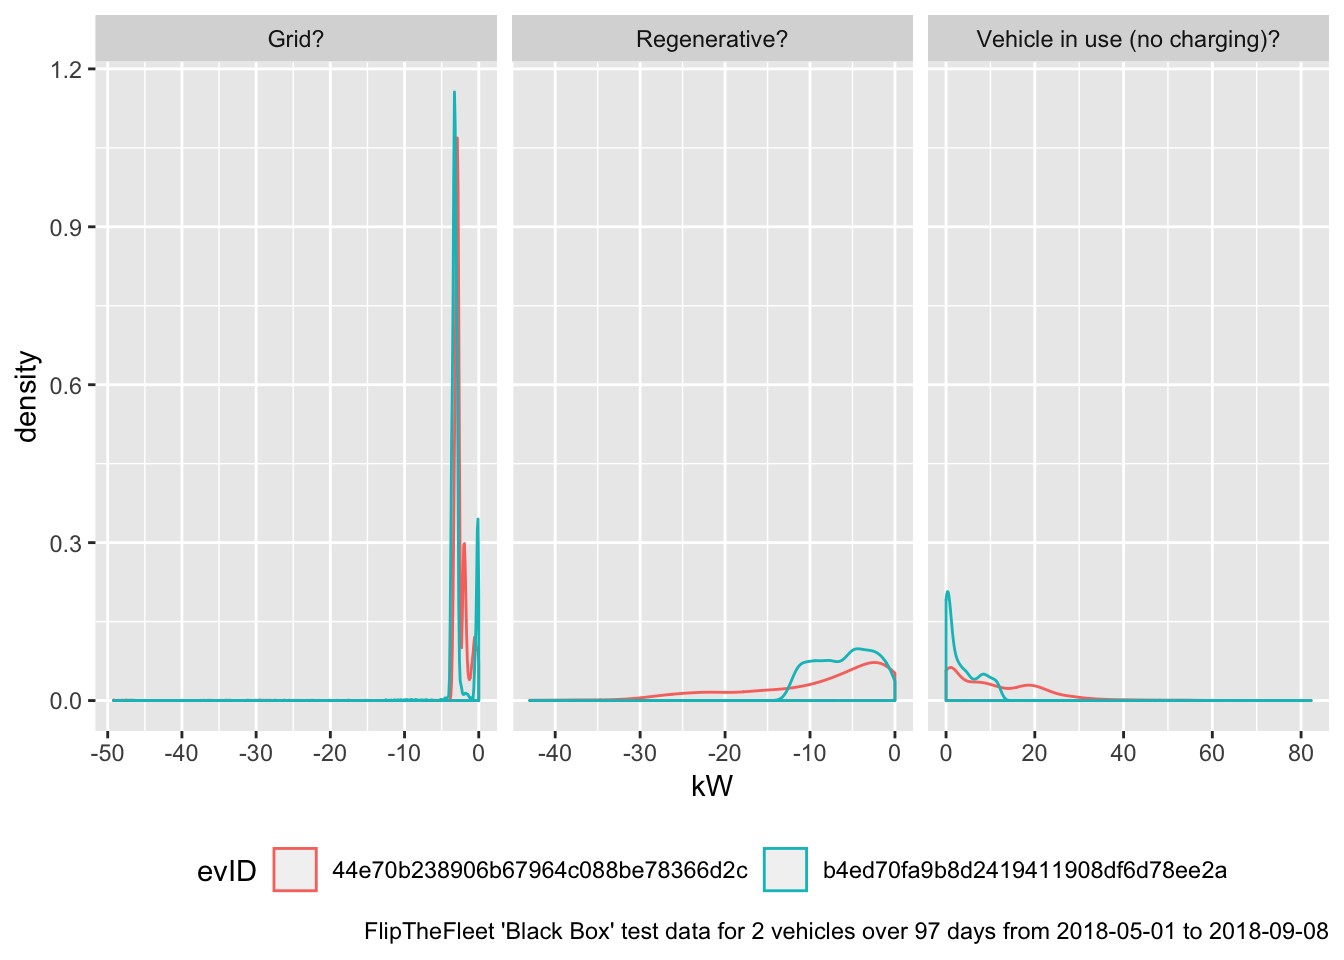
\includegraphics{ftFBlackBoxTestDataChargeTime_files/figure-latex/chargingHisto-1.pdf}

\section{Analysis: Timing of
charging}\label{analysis-timing-of-charging}

Figure \ref{fig:plotChargingTime} shows mean kW for inferred grid-based
charging by time of day over the entire test datset of 97 days from
2018-05-01 to 2018-09-08.

\begin{quote}
Does this look like what we expect?
\end{quote}

\begin{verbatim}
## Warning: Removed 268 rows containing missing values (geom_point).
\end{verbatim}

\begin{figure}
\centering
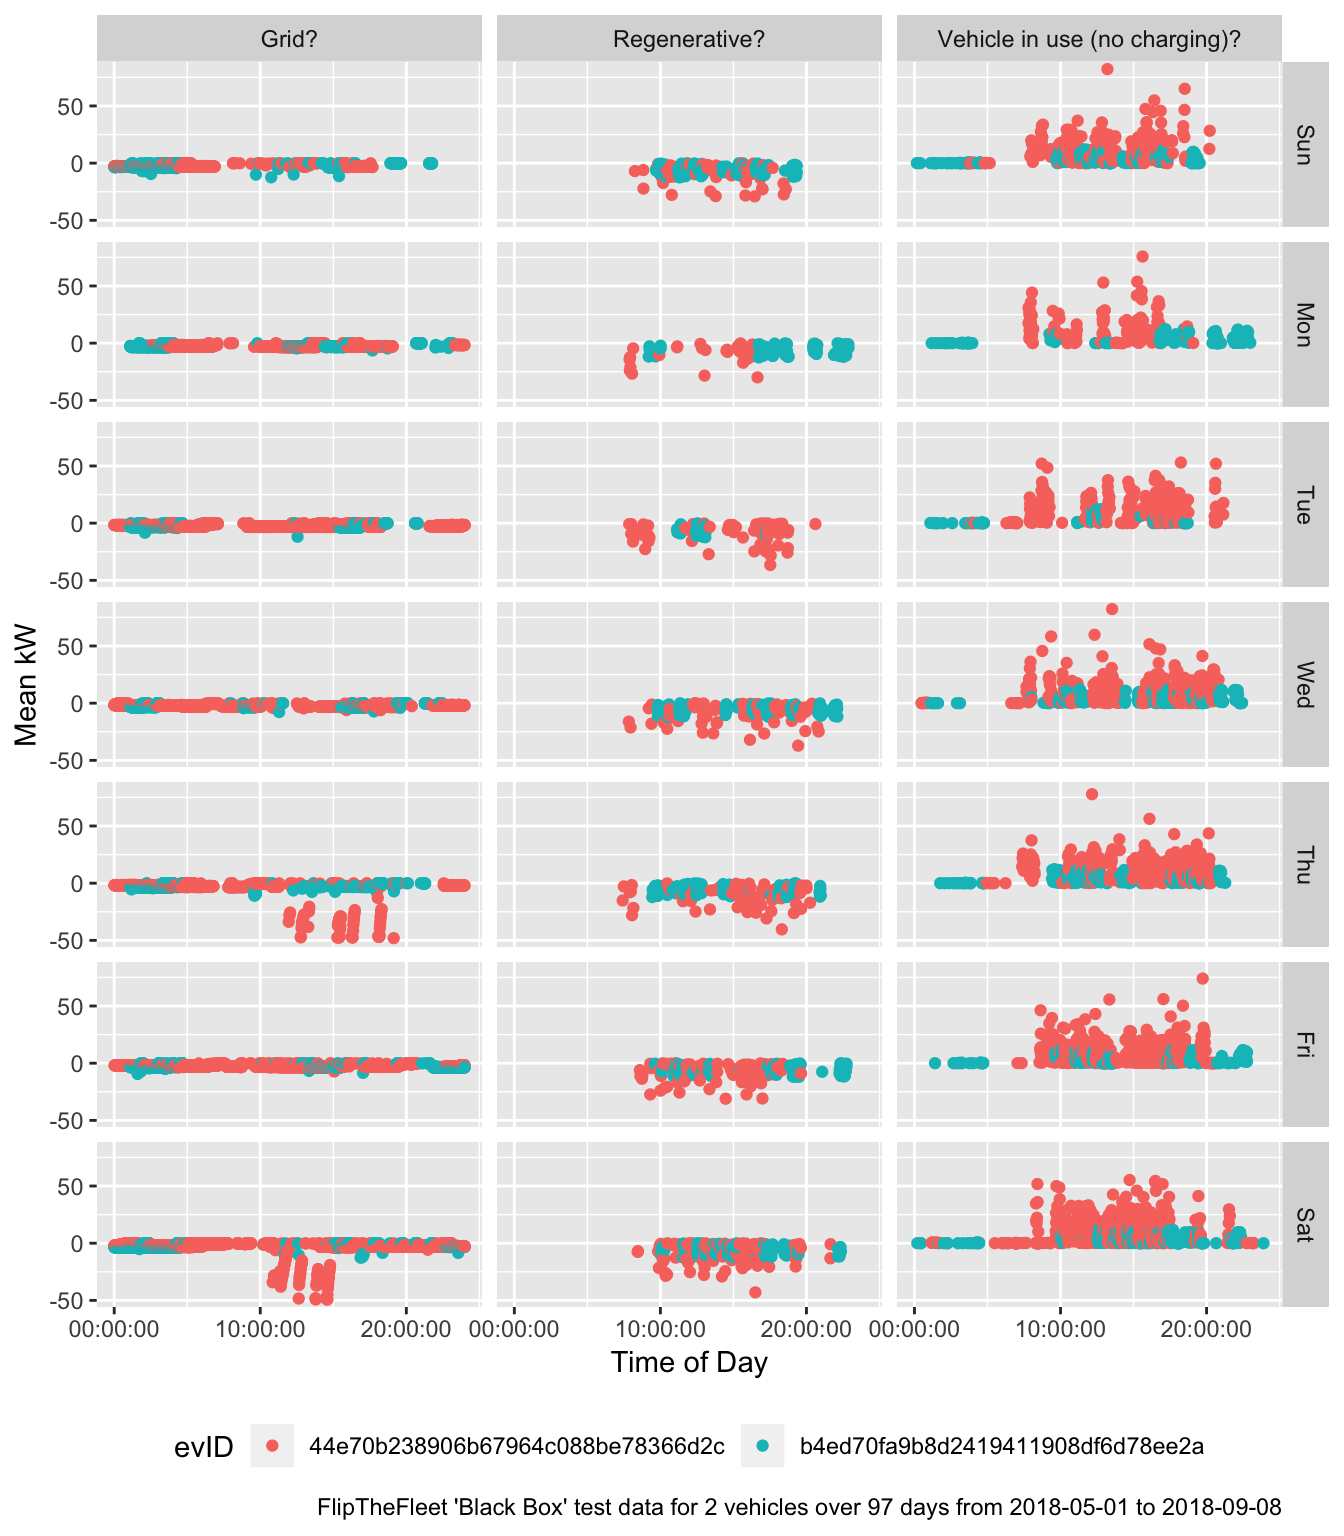
\includegraphics{ftFBlackBoxTestDataChargeTime_files/figure-latex/plotChargingTime-1.pdf}
\caption{\label{fig:plotChargingTime}Inferred charging times and power draw
(all data)}
\end{figure}

Figure \ref{fig:gridChargingTimingLine} reproduces the previous plot but
only shows the mean power flow for observations which we think are
\texttt{Grid?} charging and plots them by derived location. This
highlights a few observations with apparently large power flows - is
this fast charging or instrument error?

\begin{figure}
\centering
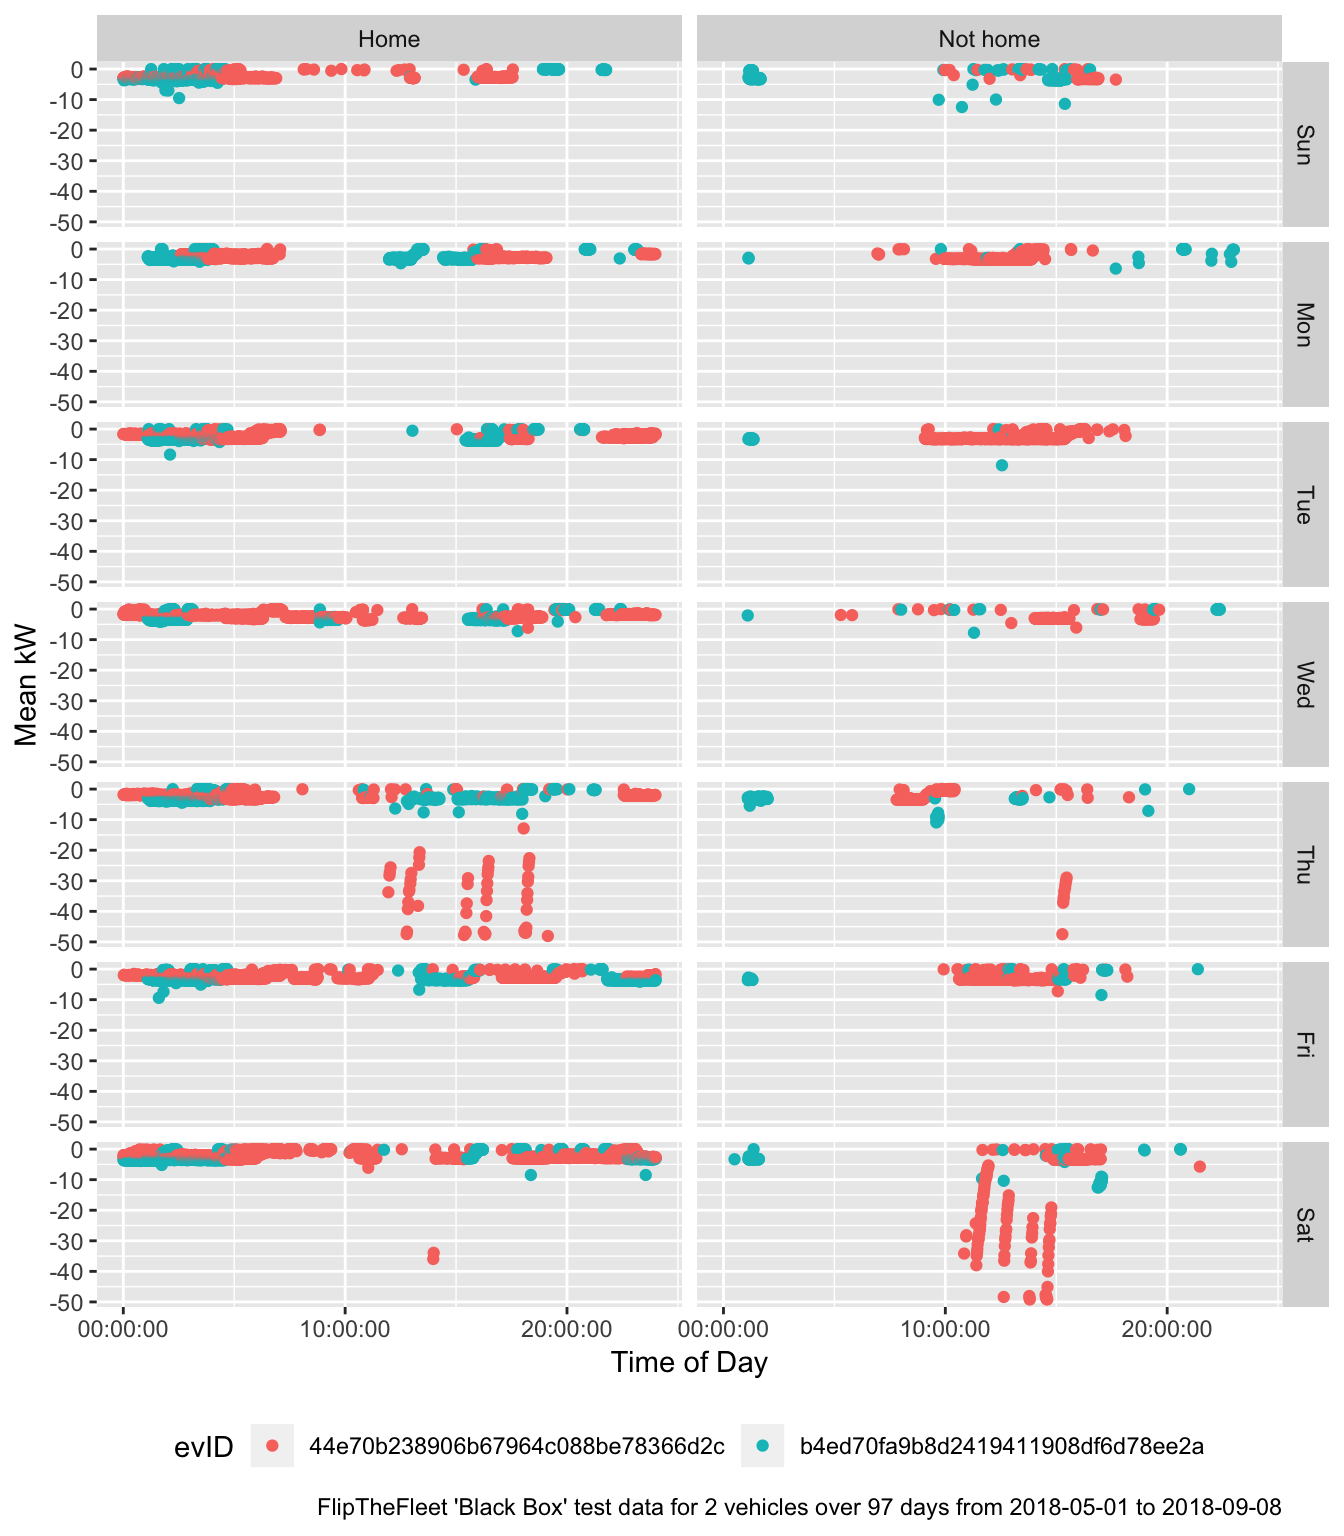
\includegraphics{ftFBlackBoxTestDataChargeTime_files/figure-latex/gridChargingTimingLine-1.pdf}
\caption{\label{fig:gridChargingTimingLine}Timing of power flow (all)}
\end{figure}

Finally, \ref{fig:gridChargingTimingTile} shows the mean power flow by
time of day and derived location using a tile plot with notional peak
electricity demand periods marked. This visually masks rare events such
as the large power flows and suggests charging timing patterns that make
sense?

\begin{figure}
\centering
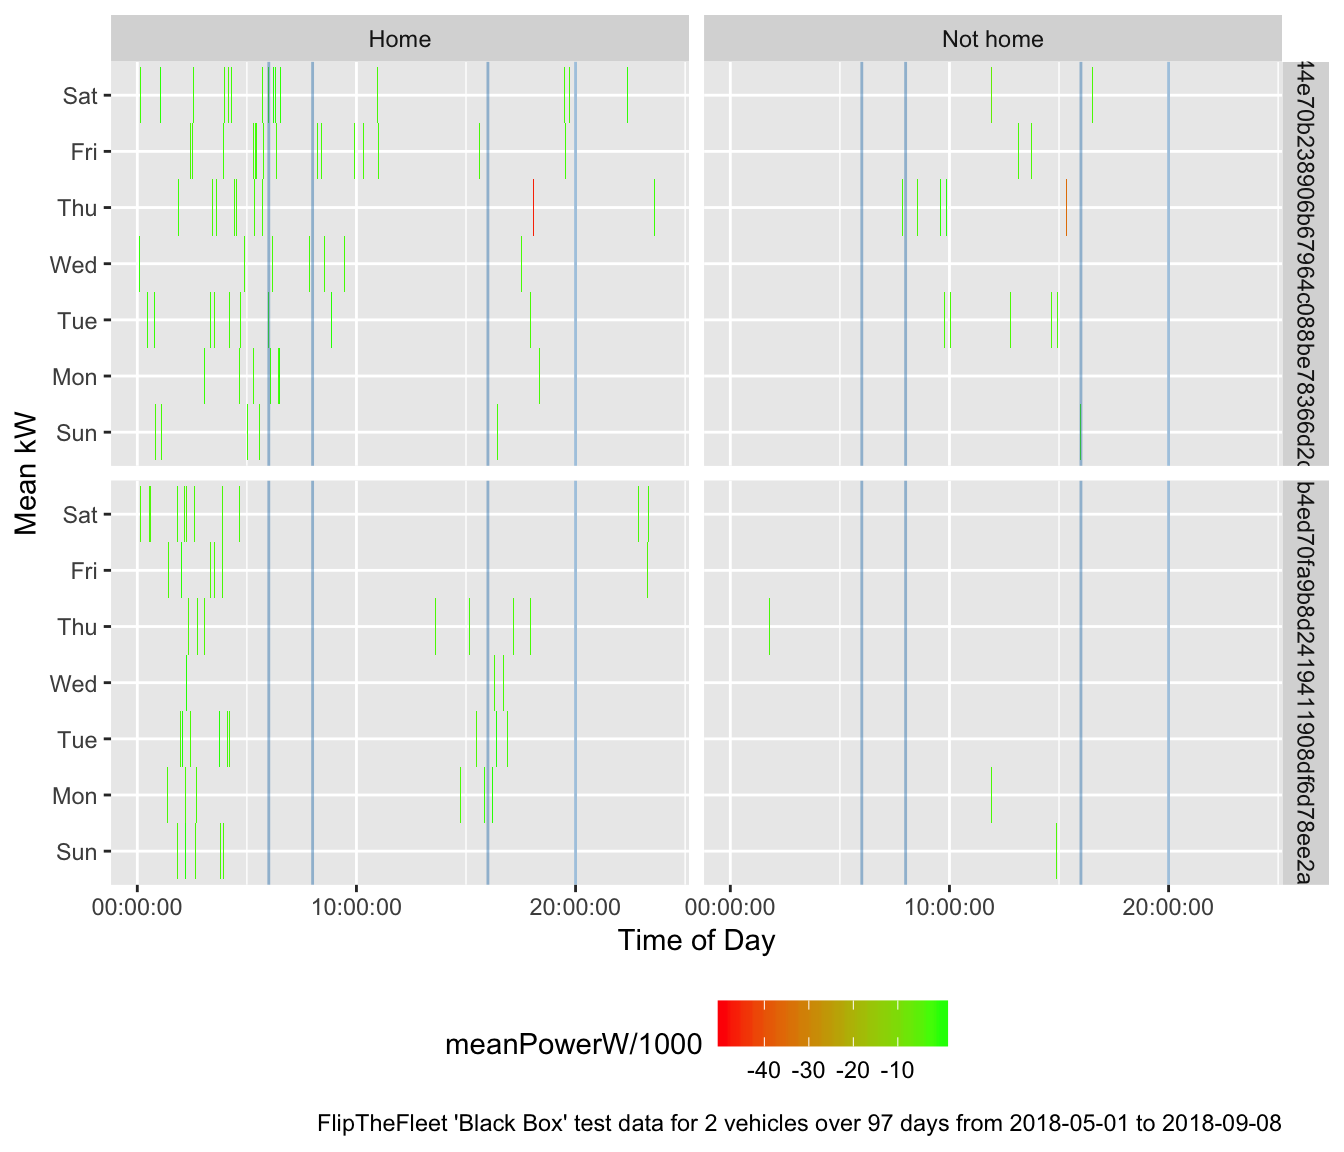
\includegraphics{ftFBlackBoxTestDataChargeTime_files/figure-latex/gridChargingTimingTile-1.pdf}
\caption{\label{fig:gridChargingTimingTile}Timing of charging from the grid}
\end{figure}

\section{Conclusions}\label{conclusions}

Questions to be asked

\begin{itemize}
\tightlist
\item
  Data:

  \begin{itemize}
  \tightlist
  \item
    Do the Amp \& Volt distributions look right?
  \item
    Cause of Pack amp \& Pack volt outliers?
  \item
    Date/Time NA (37.38 \% of observations) are due to a lack of GPS
    date/time (and lat/long). Does this mean that there is no date/time
    in the data when GPS has no signal? Our tests suggest that other
    data (e.g.~power etc) is logged even though there is no date/time.
    Do we need another source of date/time? Could we infer time from
    seconds since powered on (assumes GPS OK at start-up?)?
  \end{itemize}
\item
  Research:

  \begin{itemize}
  \tightlist
  \item
    Do all FlipTheFleet EV owners charge like this?
  \item
    Where are the EVs being charged when not at home and how can we
    tell?
  \item
    Does it vary by car/tariff/commute pattern/main use?
  \item
    What other patterns exist and how much within-vehicle and
    between-vehicle variation is there?
  \end{itemize}
\end{itemize}

\section{Runtime}\label{runtime}

Analysis completed in 11.42 seconds ( 0.19 minutes) using
\href{https://cran.r-project.org/package=knitr}{knitr} in
\href{http://www.rstudio.com}{RStudio} with R version 3.5.1 (2018-07-02)
running on x86\_64-apple-darwin15.6.0.

\section{R environment}\label{r-environment}

R packages used:

\begin{itemize}
\tightlist
\item
  base R - for the basics (R Core Team 2016)
\item
  data.table - for fast (big) data handling (Dowle et al. 2015)
\item
  lubridate - date manipulation (Grolemund and Wickham 2011)
\item
  ggplot2 - for slick graphics (Wickham 2009)
\item
  readr - for csv reading/writing (Wickham, Hester, and Francois 2016)
\item
  openssl - for hashing \texttt{Reg\ No} (Ooms 2018)
\item
  knitr - to create this document \& neat tables (Xie 2016)
\item
  GREENGrid - for local NZ GREEN Grid project utilities
\end{itemize}

Session info:

\begin{verbatim}
## R version 3.5.1 (2018-07-02)
## Platform: x86_64-apple-darwin15.6.0 (64-bit)
## Running under: macOS High Sierra 10.13.6
## 
## Matrix products: default
## BLAS: /Library/Frameworks/R.framework/Versions/3.5/Resources/lib/libRblas.0.dylib
## LAPACK: /Library/Frameworks/R.framework/Versions/3.5/Resources/lib/libRlapack.dylib
## 
## locale:
## [1] en_NZ.UTF-8/en_NZ.UTF-8/en_NZ.UTF-8/C/en_NZ.UTF-8/en_NZ.UTF-8
## 
## attached base packages:
## [1] stats     graphics  grDevices utils     datasets  methods   base     
## 
## other attached packages:
##  [1] kableExtra_0.9.0   GREENGrid_0.1.0    skimr_1.0.3       
##  [4] codebook_0.6.3     Hmisc_4.1-1        Formula_1.2-3     
##  [7] survival_2.42-3    lattice_0.20-35    readr_1.1.1       
## [10] lubridate_1.7.4    ggplot2_3.0.0      dplyr_0.7.6       
## [13] data.table_1.11.8  dkUtils_0.0.0.9000
## 
## loaded via a namespace (and not attached):
##  [1] httr_1.3.1          viridisLite_0.3.0   splines_3.5.1      
##  [4] shiny_1.1.0         assertthat_0.2.0    highr_0.7          
##  [7] latticeExtra_0.6-28 yaml_2.2.0          pillar_1.3.0       
## [10] backports_1.1.2     glue_1.3.0          digest_0.6.17      
## [13] RColorBrewer_1.1-2  promises_1.0.1      checkmate_1.8.5    
## [16] rvest_0.3.2         colorspace_1.3-2    htmltools_0.3.6    
## [19] httpuv_1.4.5        Matrix_1.2-14       plyr_1.8.4         
## [22] pkgconfig_2.0.2     labelled_1.1.0      haven_1.1.2        
## [25] bookdown_0.7        purrr_0.2.5         xtable_1.8-3       
## [28] scales_1.0.0        jpeg_0.1-8          later_0.7.5        
## [31] htmlTable_1.12      tibble_1.4.2        openssl_1.0.2      
## [34] withr_2.1.2         nnet_7.3-12         lazyeval_0.2.1     
## [37] cli_1.0.1           magrittr_1.5        crayon_1.3.4       
## [40] mime_0.5            evaluate_0.11       fansi_0.4.0        
## [43] forcats_0.3.0       xml2_1.2.0          foreign_0.8-70     
## [46] tools_3.5.1         hms_0.4.2           stringr_1.3.1      
## [49] munsell_0.5.0       cluster_2.0.7-1     bindrcpp_0.2.2     
## [52] compiler_3.5.1      rlang_0.2.2         grid_3.5.1         
## [55] rstudioapi_0.8      htmlwidgets_1.3     miniUI_0.1.1.1     
## [58] labeling_0.3        base64enc_0.1-3     rmarkdown_1.10     
## [61] gtable_0.2.0        reshape2_1.4.3      R6_2.3.0           
## [64] gridExtra_2.3       knitr_1.20          utf8_1.1.4         
## [67] bindr_0.1.1         rprojroot_1.3-2     stringi_1.2.4      
## [70] Rcpp_0.12.19        rpart_4.1-13        acepack_1.4.1      
## [73] tidyselect_0.2.4    xfun_0.3
\end{verbatim}

\section*{References}\label{references}
\addcontentsline{toc}{section}{References}

\hypertarget{refs}{}
\hypertarget{ref-data.table}{}
Dowle, M, A Srinivasan, T Short, S Lianoglou with contributions from R
Saporta, and E Antonyan. 2015. \emph{Data.table: Extension of
Data.frame}. \url{https://CRAN.R-project.org/package=data.table}.

\hypertarget{ref-lubridate}{}
Grolemund, Garrett, and Hadley Wickham. 2011. ``Dates and Times Made
Easy with lubridate.'' \emph{Journal of Statistical Software} 40 (3):
1--25. \url{http://www.jstatsoft.org/v40/i03/}.

\hypertarget{ref-openssl}{}
Ooms, Jeroen. 2018. \emph{Openssl: Toolkit for Encryption, Signatures
and Certificates Based on Openssl}.
\url{https://CRAN.R-project.org/package=openssl}.

\hypertarget{ref-baseR}{}
R Core Team. 2016. \emph{R: A Language and Environment for Statistical
Computing}. Vienna, Austria: R Foundation for Statistical Computing.
\url{https://www.R-project.org/}.

\hypertarget{ref-ggplot2}{}
Wickham, Hadley. 2009. \emph{Ggplot2: Elegant Graphics for Data
Analysis}. Springer-Verlag New York. \url{http://ggplot2.org}.

\hypertarget{ref-readr}{}
Wickham, Hadley, Jim Hester, and Romain Francois. 2016. \emph{Readr:
Read Tabular Data}. \url{https://CRAN.R-project.org/package=readr}.

\hypertarget{ref-knitr}{}
Xie, Yihui. 2016. \emph{Knitr: A General-Purpose Package for Dynamic
Report Generation in R}. \url{https://CRAN.R-project.org/package=knitr}.


\end{document}
